\section{Chapter Summary}
%\section{Summary}

% We introduced models to describe the transformation process from global
% geographic data to abstract feature space. We have demonstrated the
% versatility of this approach through showing its application to two very
% different domains working with different forms of data. Case study 1
% demonstrated the application of our framework to directly observed
% trajectory data of moving point objects. Case study 2 demonstrated the
% application of our framework to time-varying count data, which provides
% aggregated observations of moving point objects. In both of these case
% studies, application of our model transformation framework allowed us to
% generate domain-specific tools to cater to the spatio-temporal analysis
% needs of that domain.

% Typically, building applications for spatio-temporal analysis is a time
% consuming process involving many developers, and often involves multiple
% iterations in order to meet the client needs. Use of our model may help
% reduce the number of iterations needed, as well as offers the ability to
% design these systems in a consistent way, thus providing potential for
% code-reuse between different domains. The advantage of this goes beyond
% simply speeding up development times: cartographic transformations, if
% not well understood, are a frequent cause of distortions that undermine
% data integrity, and reduce confidence in the resulting analysis. Our
% system offers the potential for a new class of software that empowers
% novice users with the tools for cartographically sound, in-depth,
% spatio-temporal analysis of their domain.

%\section{Chapter Summary}

This chapter examined the issue of converting GPS data in latitude,~longitude coordinates to x,~y coordinates relative to the field. A tool was proposed to increase the efficiency and correctness of this process.

The \textit{GPS to XYT} tool designed in this thesis was motivated by the need to allow sport performance analysts to reproject player tracking data relative to the sport field, but is applicable to other domains, such as the animal tracking example shown in \figref{fig:animal-tracking}. The example shows a proof of concept demonstration that integrates the \textit{GPS to XYT} reference frame concept as an extension to the GeoJSON.io GIS editor\footnote{\url{http://geojson.io}}. The extension allows lines drawn in the editor to be used as reference frames and provides an ``XYT'' and ``Heat'' tab to facilitate analysis of the tracking data within the reprojected perspective defined by the reference frame. The albatross GPS tracking data used in this example was obtained form ZoaTrack.org\footnote{Thomas, B, Minot, E (2016) Data from: `Fledging behaviour of juvenile northern royal albatrosses (Diomedea sanfordi): a GPS tracking study'. ZoaTrack.org. doi: \url{http://dx.doi.org/10.4226/68/5733FAA628046}}.

\begin{figure*}
%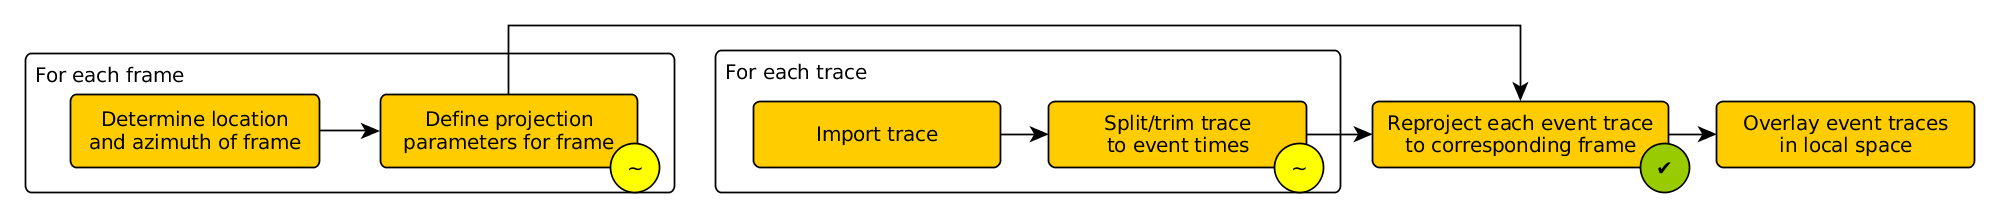
\includegraphics[width=1.0\textwidth]{figs/paper/manual-process}
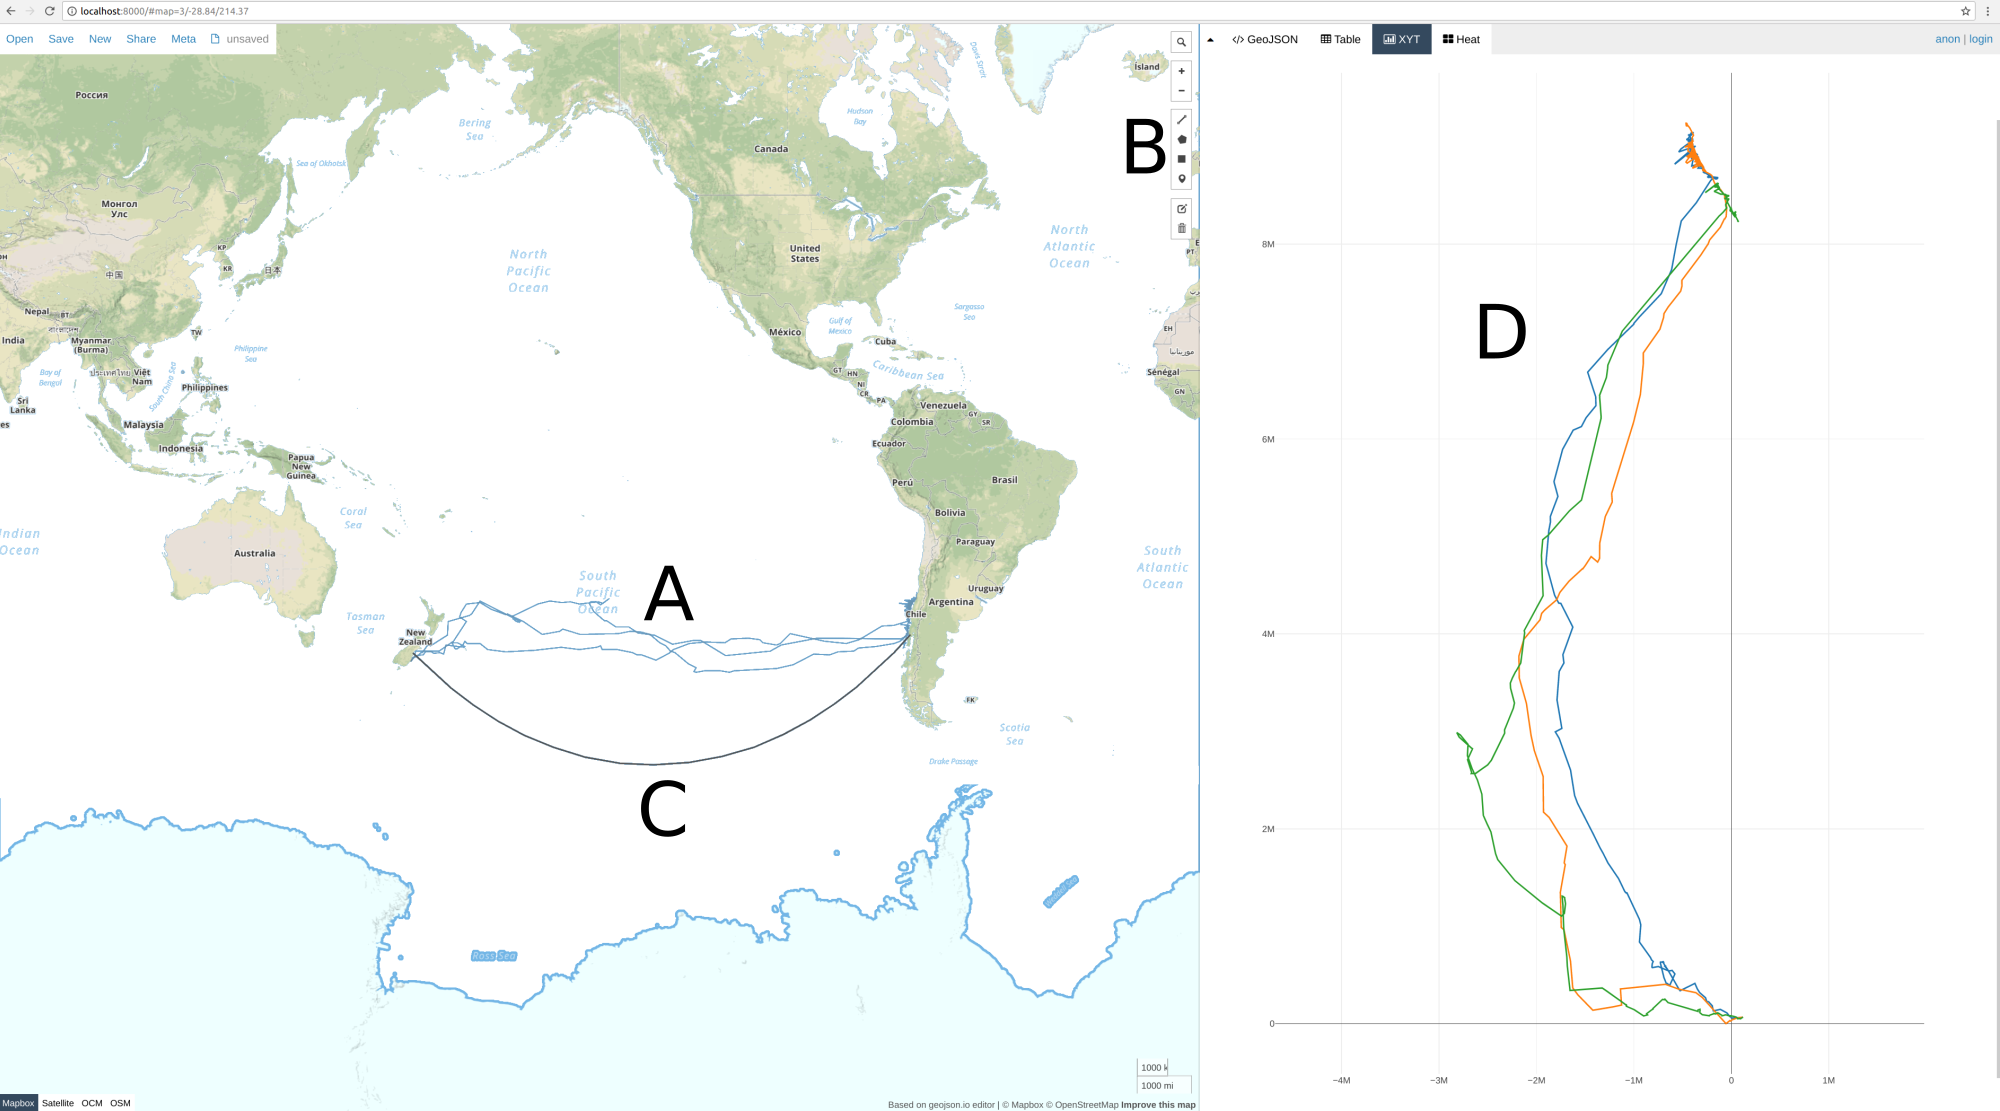
\includegraphics[width=1.0\linewidth]{figs/screenshot-xyt-annotation-export.png}
\caption{A) Migration paths of three albatrosses from New Zealand to Chile as viewed on map using Mercator projection. B) The user constructs a reference frame by using the GIS editor tools to draw a line starting at New Zealand and ending at Chile. C) The constructed line is the shortest path, which is via the Subantarctic. This appears curved on the Mercator projection. D) The \textit{GPS to XYT} tool reprojects each of the paths taken by the albatrosses relative to the reference frame line constructed by the user. In contrast to the Mercator projection, is evident from the reprojected paths that all three albatrosses deviated from the shortest path, instead preferring to take the longer path due east.}
\label{fig:animal-tracking}
\end{figure*}

Typically, building applications for spatio-temporal analysis is a time
consuming process involving many developers, and often involves multiple
iterations in order to meet the client needs. Use of the proposed solution may help
reduce the number of iterations needed, as well as offer the ability to
design these systems in a consistent way, thus providing potential for
code-reuse between different domains. The advantage of this goes beyond
simply speeding up development times: cartographic transformations, if
not well understood, are a frequent cause of distortions that undermine
data integrity, and reduce confidence in the resulting analysis. The proposed
system empowers novice users with the tools for cartographically sound
spatio-temporal analysis of their domain.

\subsection*{Applications to Sport}

\begin{figure*}
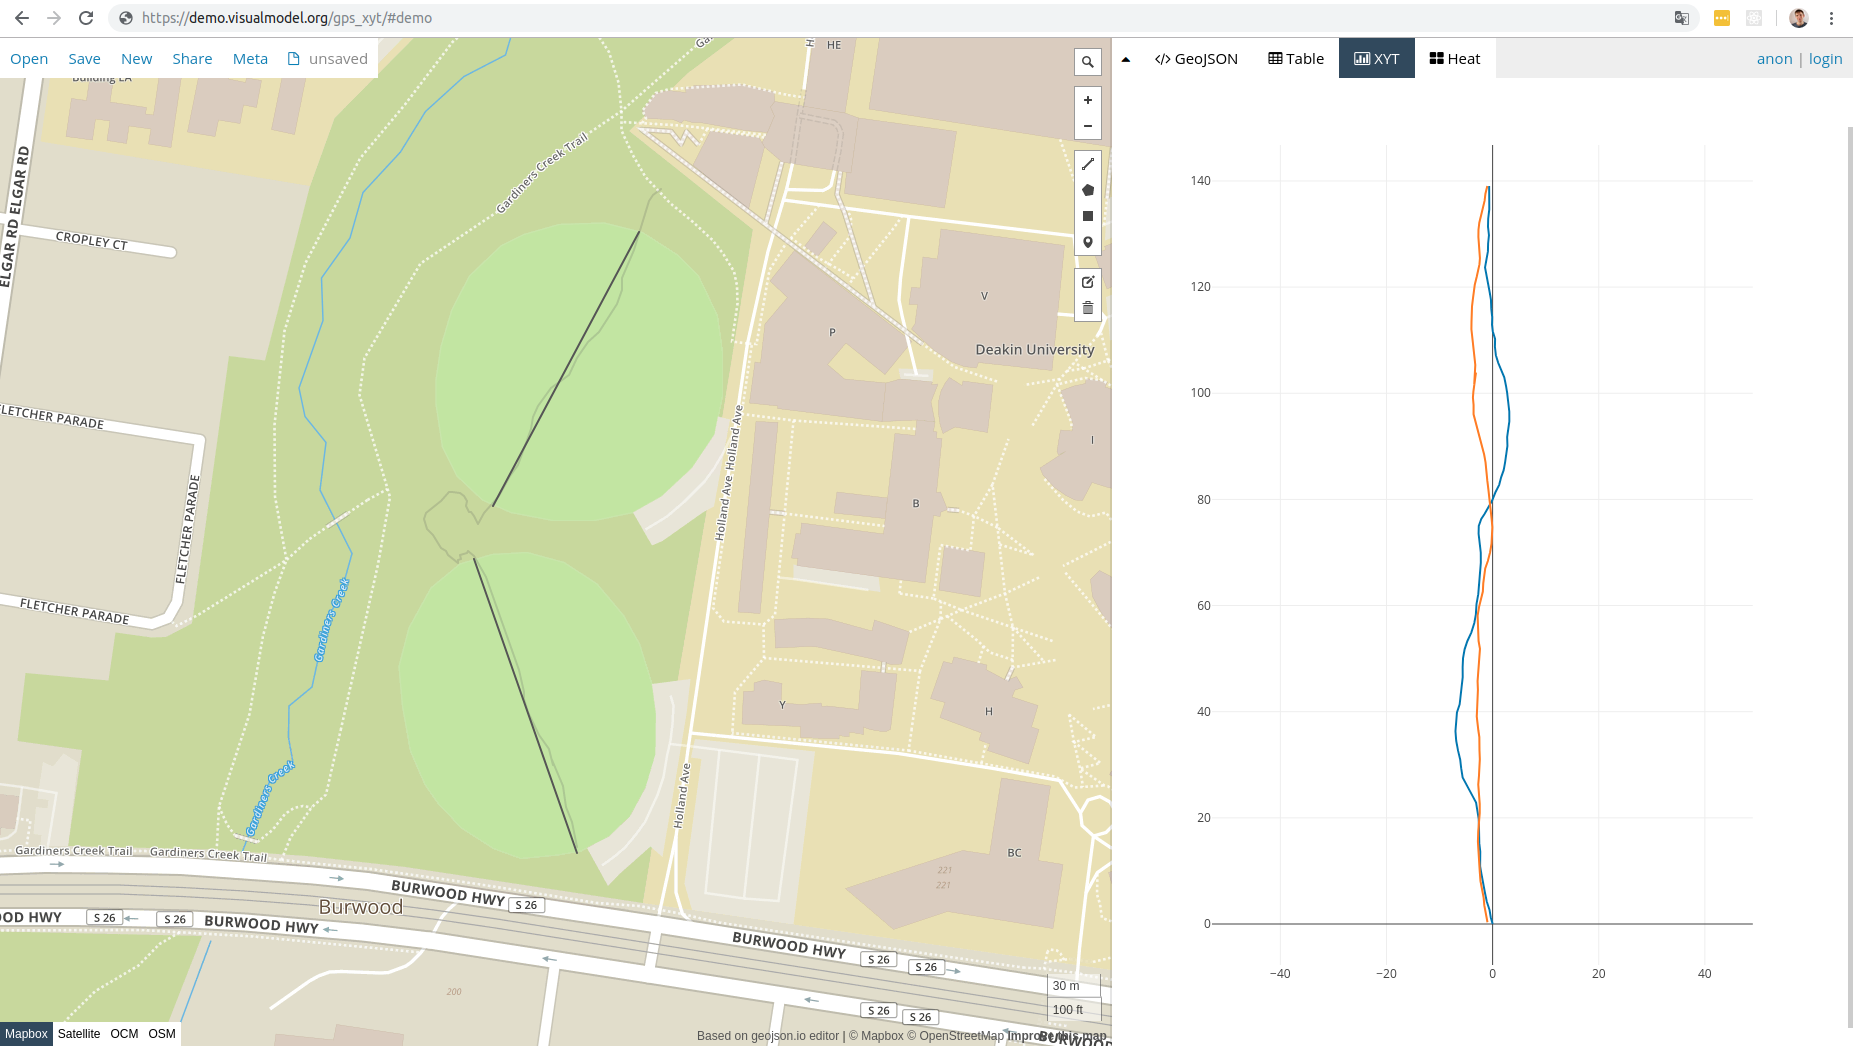
\includegraphics[width=1.0\linewidth]{figs/screenshot-xyt-demo-vismodel.png}
\caption{Use of the \textit{GPS to XYT} tool to inspect a sample GPS trajectory walking across the sport fields at Deakin University. The interface makes it easy to set up coordinate systems for each of the fields by drawing lines in the editor. The trajectory is automatically split and reprojected with respect to field coordinates to facilitate comparison, as displayed on the right hand side.}
\label{fig:xyt-demo-vismodel}
\end{figure*}

\figref{fig:xyt-demo-vismodel} shows an example of using the interactive \textit{GPS to XYT} tool (implemented as an extension to the to GeoJSON.io GIS editor) to inspect a sample GPS trace. The sample GPS trace was captured using a mobile phone GPS; however, the same procedure can be applied to data from professional sport devices after converting them to a standard data format. An extended command line version of the \textit{GPS to XYT} tool was used in \secref{sec:integration-reprojection} to reproject the sport player GPS tracking data analysed in this thesis.

\subsection*{Future Work}

Future work is necessary to evaluate our system with sport performance analysts. While the system was theoretically shown in \secref{sec:sigspatialeval} to reduce the number of user steps required, and was argued to reduce the level of knowledge required to use the system according to Bloom's revised taxonomy, an empirical evaluation is needed to confirm whether these theoretical advantages correspond to faster use and lower error rates on real-world tasks.

\subsection*{Contributions}

\begin{enumerate}
%  \item Built up a domain model of consistent AFL terminology and holistic understanding of the game state.
  \item Proposed a novel method for representing spatio-temporal reference frames as geographic objects. This allows GIS novices, such as sport performance analysts, to configure reference frames without the need for deep conceptual knowledge of cartographic projections. It also facilitates partial automation (e.g. reprojecting GPS data to the closest sport field), thus resulting in time savings when the analysis involves multiple reference frames (e.g. a season of GPS tracking data involving multiple sport fields).
\end{enumerate}
